\subsection{Estructura del backend}
El servidor se organiza en módulos interconectados para ofrecer servicios robustos al frontend y facilitar un desarrollo escalable.
Una petición HTTP sigue esta secuencia: el cliente consume una ruta (endpoint), se ejecutan los middlewares de autenticación y/o carga de imágenes si corresponde, y un controlador procesa los datos interactuando con uno o varios modelos para luego devolver la respuesta que corresponda. Por ello, se distinguen los siguientes modulos principales:

\begin{itemize}
    \item \textbf{Entrada y Configuración Inicial}: En la raíz del proyecto se encuentra el archivo \texttt{index.js}, encargado de configurar y levantar el servidor. Para ello, se conecta a la base de datos y carga los endpoints y los middlewares pertinentes.

    Para que el frontend tenga acceso a la API, es esencial configurar el mecanismo de seguridad \textbf{CORS (Cross-Origin Resource Sharing)}. En una arquitectura desacoplada como la de este proyecto, el cliente y el servidor suelen operar en dominios o puertos distintos. Por seguridad, los navegadores modernos aplican la "Política de Mismo Origen" (\textit{Same-Origin Policy}), que prohíbe que un script cargado en un origen acceda a recursos de otro distinto. Con la configuración de \texttt{CORS} se define una lista de dominios autorizados a acceder a la API, así como habilitar el intercambio de credenciales.

    \begin{figure}[h]
    \centering
    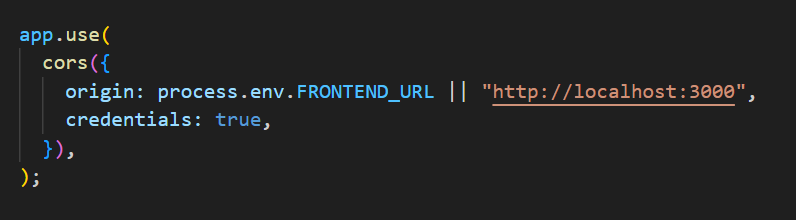
\includegraphics[width=0.8\textwidth]{imagenes/cors.png}
    \caption{Configuración del CORS en la entrada del backend}
    \label{fig:cors}
    \end{figure}

    \item \textbf{Lógica de negocio}: la lógica de negocio se organiza en una estructura con tres partes, basándose en el principio de separación por responsabilidades ("SoC" o Separation of Concerns), que busca dividir sistemas complejos en partes más pequeñas y manejables cada una de las cuales cubre una funcionalidad. Así, tenemos la definición de los puntos de acceso (\texttt{routes/}), la implementación de las reglas de negocio (\texttt{controllers/}) y la definición de los modelos de datos (\texttt{models/}).

    \item \textbf{Middlewares}: La carpeta (\texttt{middlewares/}) incluye las configuraciones de autenticación de usuario y de subida de archivos, que se explicarán en detalle más adelante.
\end{itemize}

Además, el proyecto cuenta con la carpeta \texttt{templates/}, que contiene la plantilla para enviar correos automatizados; y la carpeta \texttt{uploads/profile\_pictures/}, que actúa como almacenamiento local para las imágenes de perfil de los usuarios.


Esta separación garantiza que el sistema sea escalable y fácil de mantener.